% $Header$

\documentclass{beamer}

% This file is a solution template for:

% - Talk at a conference/colloquium.
% - Talk length is about 20min.
% - Style is ornate.



% Copyright 2004 by Till Tantau <tantau@users.sourceforge.net>.
%
% In principle, this file can be redistributed and/or modified under
% the terms of the GNU Public License, version 2.
%
% However, this file is supposed to be a template to be modified
% for your own needs. For this reason, if you use this file as a
% template and not specifically distribute it as part of a another
% package/program, I grant the extra permission to freely copy and
% modify this file as you see fit and even to delete this copyright
% notice. 


%\mode<presentation>
%{
%  \usetheme{Warsaw}
%  % or ...
%
%  \setbeamercovered{transparent}
%  % or whatever (possibly just delete it)
%}
%
%
%\usepackage[english]{babel}
%% or whatever
%
%\usepackage[latin1]{inputenc}
%% or whatever
%
%\usepackage{times}
%\usepackage[T1]{fontenc}
%% Or whatever. Note that the encoding and the font should match. If T1
%% does not look nice, try deleting the line with the fontenc.




% Setup appearance:
\mode<presentation>
{
\usetheme{Darmstadt}
\usefonttheme[onlylarge]{structurebold}
\setbeamerfont*{frametitle}{size=\normalsize,series=\bfseries}
\setbeamertemplate{navigation symbols}{}
\usefonttheme{professionalfonts}
}

% Standard packages

\usepackage[english]{babel}
\usepackage[latin1]{inputenc}
\usepackage{times}
\usepackage[T1]{fontenc}

%
%\usefonttheme[onlymath]{serif}


% Setup TikZ

\usepackage{tikz}
\usetikzlibrary{arrows}
\tikzstyle{block}=[draw opacity=0.7,line width=1.4cm]




\title[AUV control without linear velocity measurements] % (optional, use only with long paper titles)
{Inertial-aided Homography-based Visual Servo Control of Autonomous Underwater Vehicles without Linear Velocity Measurements}

%\subtitle
%{Include Only If Paper Has a Subtitle}

%\author[Author, Another] % (optional, use only with lots of authors)
%{F.~Author\inst{1} \and S.~Another\inst{2}}
% - Give the names in the same order as the appear in the paper.
% - Use the \inst{?} command only if the authors have different
%   affiliation.

%\institute[Universities of Somewhere and Elsewhere] % (optional, but mostly needed)
%{
%  \inst{1}%
% Department of Computer Science\\
% University of Somewhere
% \and
%  \inst{2}%
%  Department of Theoretical Philosophy\\
%  University of Elsewhere}
% - Use the \inst command only if there are several affiliations.
% - Keep it simple, no one is interested in your street address.

\author[Nguyen, Hua, Allibert and Hamel] % (optional, use only with lots of authors)
{L.-H.~Nguyen \and M.-D.~Hua \and G.~Allibert \and T.~Hamel}
\institute[Universities of Somewhere and Elsewhere] % (optional, but mostly needed)
{
	\textit{I3S Laboratory, CNRS, Universit\'e C\^ote d'Azur}\\
	Sophia Antipolis, France \\
	lhnguyen(hua,allibert,thamel)@i3s.unice.fr}
	
	
\date[ICSTCC 2017] % (optional, should be abbreviation of conference name)
{21$^{st}$ ICSTCC, October 19 - 21, 2017, Sinaia, Romania}
% - Either use conference name or its abbreviation.
% - Not really informative to the audience, more for people (including
%   yourself) who are reading the slides online

%\subject{Theoretical Computer Science}
% This is only inserted into the PDF information catalog. Can be left
% out. 



% If you have a file called "university-logo-filename.xxx", where xxx
% is a graphic format that can be processed by latex or pdflatex,
% resp., then you can add a logo as follows:

 %\pgfdeclareimage[height=0.5cm]{university-logo}{Images/university.png}
% \logo{\pgfuseimage{university-logo}}

\titlegraphic{
\includegraphics[width=0.9cm]{Images/cnrs_transparent.png}\hspace*{2.8cm}~%
	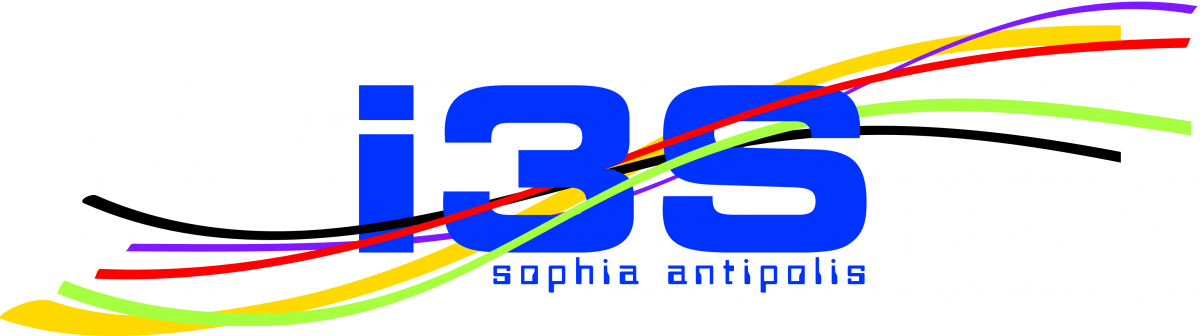
\includegraphics[width=3cm]{Images/NewlogoI3S.png}\hspace*{1.0cm}~
	
\includegraphics[width=3cm]{Images/university.png}}

% Delete this, if you do not want the table of contents to pop up at
% the beginning of each subsection:
\AtBeginSubsection[]
{
  \begin{frame}<beamer>{Outline}
    \tableofcontents[currentsection,currentsubsection]
  \end{frame}
}


% If you wish to uncover everything in a step-wise fashion, uncomment
% the following command: 

%\beamerdefaultoverlayspecification{<+->}


\begin{document}

\begin{frame}
  \titlepage
\end{frame}

\begin{frame}{Outline}
  \tableofcontents
  % You might wish to add the option [pausesections]
\end{frame}


% Structuring a talk is a difficult task and the following structure
% may not be suitable. Here are some rules that apply for this
% solution: 

% - Exactly two or three sections (other than the summary).
% - At *most* three subsections per section.
% - Talk about 30s to 2min per frame. So there should be between about
%   15 and 30 frames, all told.

% - A conference audience is likely to know very little of what you
%   are going to talk about. So *simplify*!
% - In a 20min talk, getting the main ideas across is hard
%   enough. Leave out details, even if it means being less precise than
%   you think necessary.
% - If you omit details that are vital to the proof/implementation,
%   just say so once. Everybody will be happy with that.

\section{Motivation}

%\subsection{The Basic Problem}

%\begin{frame}{Why Visual Servo Control is used?}
% 
%	\begin{columns}[t]
%		\column{.5\textwidth}	
%		\begin{block}{Global acoustic positioning system issues:}		
%			\begin{itemize}
%				\item Unusable
%				\item Insufficiently precise 
%			\end{itemize}
%		\end{block}
%		\pause
%		\begin{block}{Camera}		
%			\begin{itemize}
%				\item Allow operation closed to structures
%				\item Rich of information
%			\end{itemize}
%		\end{block}
%	
%		\pause
%		\column{.5\textwidth}		
%		\begin{block}{Stereo camera}
%			\begin{itemize}
%				\item Require high processing power computer
%				\item Ineffective when far from scene
%			\end{itemize}
%		\end{block}
%		\begin{block}{Monocular camera}
%			\begin{itemize}
%				\item Less demande on processing power  
%				\item More challenging  
%			\end{itemize}
%		\end{block}
%	\end{columns}
%	\begin{exampleblock}{Motivation 1:}
%		\centering
%		{\color{red} \textbf{Visual servo control using monocular camera}}
%	\end{exampleblock}
%\end{frame}

\begin{frame}{Why Visual Servo Control is used?}

\begin{columns}[t]
	\column{.4\textwidth}	
	\begin{block}{{\footnotesize Global acoustic positioning system issues:}}		
		\begin{itemize}
			\item Unusable
			\item Insufficiently precise measurements
		\end{itemize}
	\end{block}
	\pause	
	\column{.65\textwidth}
	\begin{block}{Camera}		
		\begin{itemize}
			\item Allow operation closed to structures
			\item Rich of information acquired
		\end{itemize}
		\vspace{-0.5cm}
		\begin{columns}
			\column[content...]{.5\textwidth}
			\begin{figure}	
				\centering		
				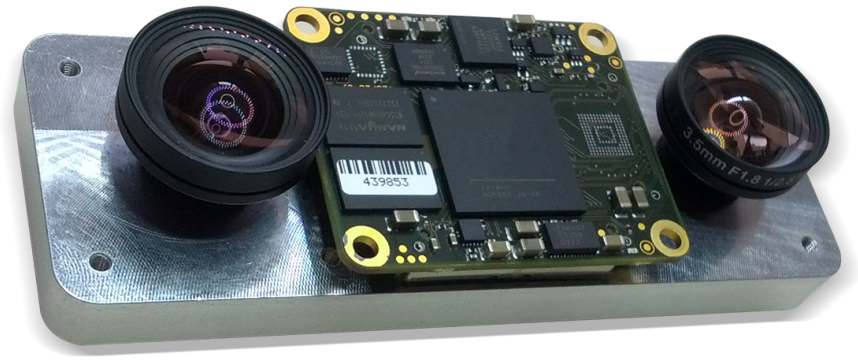
\includegraphics[width = 43mm]{Images/stereo_camera.png}\\
				{\color{blue}\tiny  https://www.autonomos-systems.de} \\
				Stereo camera
			\end{figure}
			\column[content...]{.5\textwidth}
			\begin{figure}				
				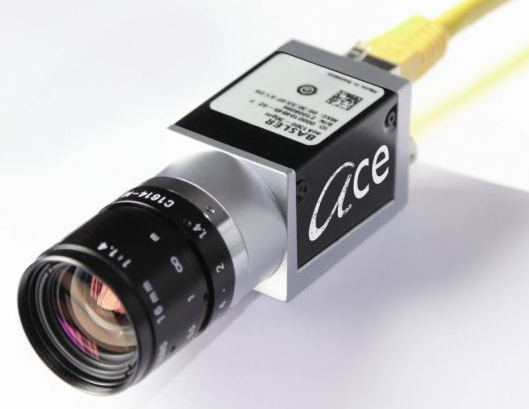
\includegraphics[width = 30mm]{Images/Monocular_camera.png}\\
				%\vspace{0.35cm}
				{\color{blue}\tiny https://www.baslerweb.com/} \\
				Monocular camera\\
			\end{figure}
			
		\end{columns}
	\end{block}	
	\end{columns}
	\pause
	\begin{exampleblock}{Motivation 1:}
		\centering
		{\color{red} \textbf{Visual servo control using monocular camera}}
	\end{exampleblock}
\end{frame}


\begin{frame}{Visual servo control using monocular camera}
	\begin{itemize}
		
		\item {\color{red} \textbf{Existing algorithms rely on linear velocity  estimation or measurement}} \\{\scriptsize  [J.-E Lots et al., 2001], [S.van der Zwaan et al., 2002], [L.Brignone et al., 2007], [S. Krupinski et al, 2012], [S. Krupinski et al, 2017]}
		\pause
		\item Linear velocity is estimated by \textbf{numerical differentiation} or measured by \textbf{Doppler Velocity Log} (DVL)
	\end{itemize}

\centering
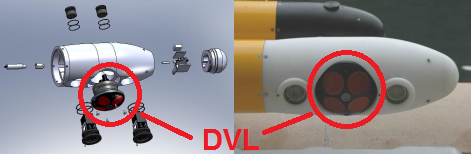
\includegraphics[width = 100mm]{Images/DVL_5.png}\\
{\footnotesize AUV nose cone housing DVL}\\
{\color{blue}\tiny Source: http://robots.engin.umich.edu}

	
		
	
 
\end{frame}


\begin{frame}{Doppler Velocity Log (DVL):}
	\vspace{-0.5cm}
	\begin{columns}[t]
		\column{.4\textwidth}
		\begin{block}{DVL issues:}
			\small
			\begin{itemize}
				\item High price \\($>$ 10K US\$)
				\item High weight
				%\item Big dimensions 
				\item Violate maximum slope-threshold of DVLs in close proximity to infrastructures
			\end{itemize}
		\end{block}
		\column{.65\textwidth}
		\begin{block}{{\small DVL comparison.} \tiny Source: Terzja van de Kuil, 2016}
			\begin{figure}
				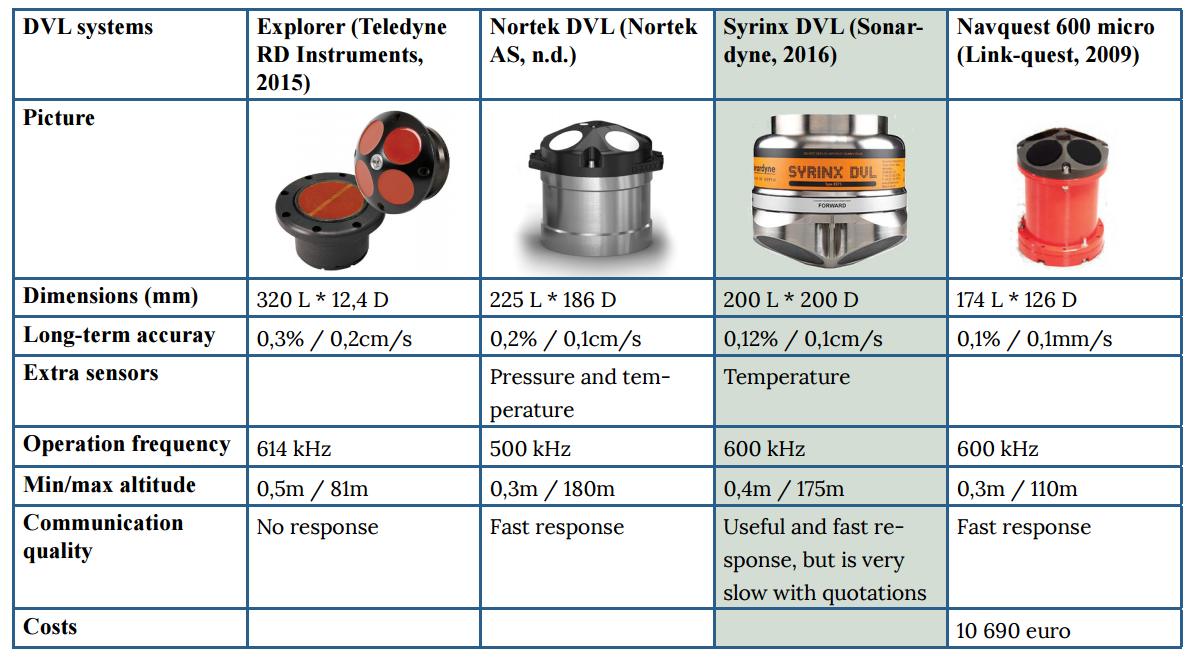
\includegraphics[width = 70mm]{Images/DVL_prices.png}\\ \vspace{0.2cm}
				{\color{blue}}
			\end{figure}
		\end{block}		
		
	\end{columns} 
\begin{exampleblock}{Motivation 2:}
	\centering
	{\color{red} \textbf{New controller without relying on linear velocity measurement ($\Rightarrow$ No need DVL)}}
\end{exampleblock}

\end{frame}

\section{System modeling \& Control design}

\begin{frame}{System modeling}
	\begin{columns}
		\column[content...]{.5\textwidth}
		\begin{figure}
			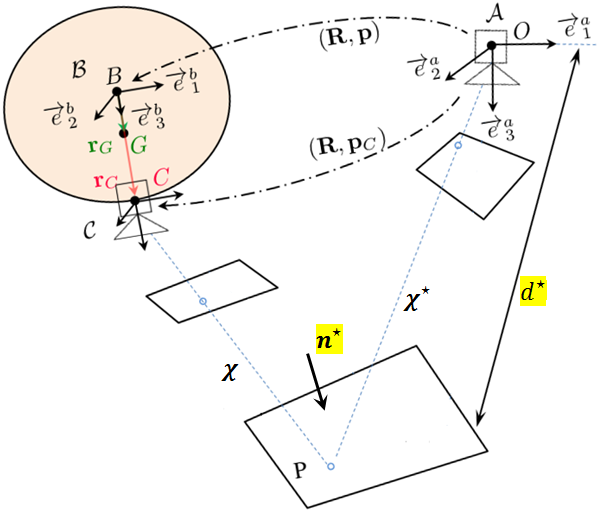
\includegraphics[width = 55mm]{Images/Notation_rot_modif3.png}
		\end{figure}
		\column[placement]{.6\textwidth}
%		\begin{block}{Assumption:}
%			\centering
%			$B,G$ and ${C}$ are aligned			%$\mathbf{B,G}$ and $\mathbf{C}$ are aligned			
%		\end{block}
		\begin{block}{Equations of motion:}
			\scriptsize \vspace{-0.4cm}
			\begin{equation*}\label{eq:system2}
			\begin{array}{rl}
			\dot{\mathbf{p}} & =  \mathbf{R} \mathbf{V} \\
			\dot{\mathbf{R}} & =  \mathbf{R} \mathbf{\Omega}_\times \\
			\!\!\dot{\mathbf{P}}_h &= \mathbf{P}_h \times \mathbf{\Omega} +\mathbf{F}_c + \mathbf{F}_{gb} + \mathbf{F}_d  \\
			\!\!\dot{\mathbf{\Pi}}_h &=  \mathbf{\Pi}_h \!\times\! \mathbf{\mathbf{\Omega}} + \underbrace{{\color{red}\mathbf{P}_h \!\times \!\mathbf{V}_h}}_{\color{red} \text{{\footnotesize Munk moment}}}  +\mathbf{\Gamma}_c + \mathbf{\Gamma}_g + \mathbf{\Gamma}_d \!\!\vspace{-0.2cm}
			\end{array}
			\end{equation*} \vspace{-0.3cm}
			%where: \\
%			\begin{equation*}
%			\begin{array}{rl}
%			\mathbf{P}_h & = \mathbf{M}\mathbf{V}_h + \mathbf{D}^{\!\top} \mathbf{\Omega}\\[1ex]
%			\mathbf{\Pi}_h & = \mathbf{J} \mathbf{\Omega} + \mathbf{D}  \mathbf{V}_h \\
%			%\mathbf{J} &\triangleq \mathbf{J}_0 +\mathbf{M}_A^{22}\\
%			\mathbf{D} &\triangleq m \mathbf{r}_{G\times} +\mathbf{M}_A^{21}
%			%\mathbf{F}_{gb}  &\triangleq (m g - F_b) \mathbf{R}^{\!\top} \mathbf{e}_3\\
%			%\mathbf{\Gamma}_g  &\triangleq mgl\mathbf{e}_{3}\! \times \!\mathbf{R}^{\!\top} \mathbf{e}_3\\
%			%\mathbf{F}_d(\mathbf{V}_h) & \triangleq - (\mathbf{D}_{V\!l}   +|\mathbf{V}_h|\mathbf{D}_{V\!q} )\mathbf{V}_h  \\
%			%\mathbf{\Gamma}_d(\mathbf{\Omega})& \triangleq  - (\mathbf{D}_{\Omega l}  + |\mathbf{\Omega}|\mathbf{D}_{\Omega q} )\mathbf{\Omega}
%			\end{array}
%			\end{equation*}
			%\begin{equation*}
			% \mathbf{M}_{A}\triangleq \begin{bmatrix} %\mathbf{M}_A^{11}  & \mathbf{M}_A^{12} \\ %\mathbf{M}_A^{21} & \mathbf{M}_A^{22}  %\end{bmatrix}, \mathbf{M}\triangleq %m\mathbf{I}_3+\mathbf{M}_A^{11}
			%\end{equation*}
%			\begin{equation*}
%			\mathbf{J} \triangleq \mathbf{J}_0 +\mathbf{M}_A^{22},\,\, \mathbf{D} \triangleq m \mathbf{r}_{G\times} +\mathbf{M}_A^{21}
%			\end{equation*}
		\end{block}
		\begin{block}{Coupling issue}
			\begin{equation*}
			\begin{array}{rl}
			\mathbf{P}_h & = \mathbf{M}\mathbf{V}_h + \mathbf{\color{red} D}^{\!\top} \mathbf{\Omega}\\[1ex]
			\mathbf{\Pi}_h & = \mathbf{J} \mathbf{\Omega} + \mathbf{\color{red} D}  \mathbf{V}_h \\
			%\mathbf{J} &\triangleq \mathbf{J}_0 +\mathbf{M}_A^{22}\\
			\mathbf{\color{red}D} &\triangleq m \mathbf{r}_{G\times} +\mathbf{M}_A^{21}
			\end{array}
			\end{equation*}
		\end{block}
	\end{columns}

\end{frame}


\begin{frame}{Model for control design}
\begin{columns}
	\column[content...]{0.4\textwidth}
	\begin{block}{Simplifications:}
		\begin{itemize}
			\scriptsize
			\item Terms relating to coupling matrix $\mathbf{D} \triangleq m \mathbf{r}_{G\times} + \mathbf{M}_A^{21}$
			\begin{itemize}
				\scriptsize
				\item Compact-shape AUVs
				\item Small distance BG
				\item Light weight AUVs
			\end{itemize}
			\item "Munk moment" $\mathbf{P}_h \!\times \!\mathbf{V}_h$
			\item Terms relating to $\mathbf{V}_f$
		\end{itemize}		
	\end{block}
	\begin{block}{Compact-shape AUV}
		\begin{figure}
			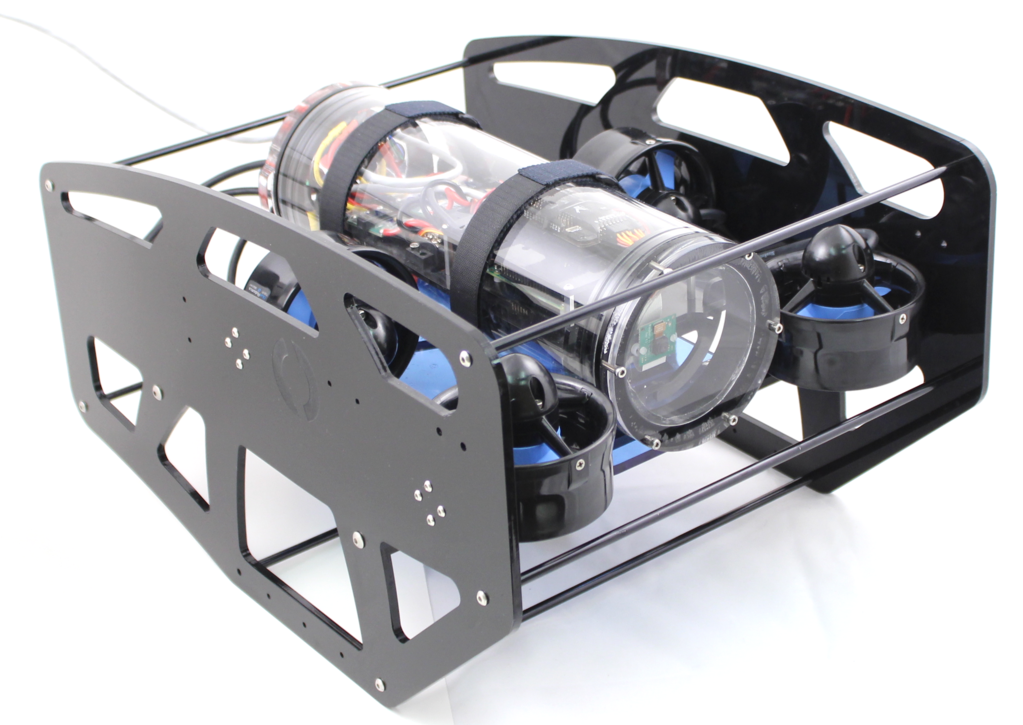
\includegraphics[width = 0.8\textwidth]{Images/Bluerov_modif.png}\\
			\tiny {\color{blue} Source: www.bluerobotics.com}
		\end{figure}
	\end{block}
	\column[content...]{0.60\textwidth}
	\pause
	\begin{block}{Model for control design}
		\scriptsize \vspace{-0.3cm}
		\[
		\begin{array}{rl}
		\dot{\mathbf{p}} & =  \mathbf{R} \mathbf{V} \label{eq:kinematicsPos}\\
		\dot{\mathbf{R}} & =  \mathbf{R} \mathbf{\Omega}_\times \\
		\mathbf{M}\dot{\mathbf{V}} &= (\mathbf{M}\mathbf{V}) \!\times\!\mathbf{\Omega} + \mathbf{F}_c + \mathbf{F}_{gb} + \mathbf{F}_d(\mathbf{V}) +{\color{red}\mathbf{\Delta}_F}  \\
		\mathbf{J}\dot{\mathbf{\Omega}} &=  (\mathbf{J}\mathbf{\Omega}) \!\times\! \mathbf{\mathbf{\Omega}} + \mathbf{\Gamma}_c + \mathbf{\Gamma}_g +  {\color{red}\mathbf{\Delta}_{\Gamma}}
		\end{array} 
		\]
		
		
		\noindent with the ``\textbf{\color{red} disturbance}'' terms: 
		\[
		\begin{array}{rl}
		{\color{red}\mathbf{\Delta}_F} \triangleq\!\!\!\!\!\!& -(\mathbf{M}\mathbf{V}_f)_\times \mathbf{\Omega} -\mathbf{M} \mathbf{\Omega}_\times \mathbf{V}_f + (\mathbf{D}^\top \mathbf{\Omega})_\times \mathbf{\Omega}\\
		&-\mathbf{D}^\top \dot{\mathbf{\Omega}}
		+ \mathbf{F}_d(\mathbf{V}_h) - \mathbf{F}_d(\mathbf{V}) \\
		{\color{red}\mathbf{\Delta}_{\Gamma}} \triangleq\!\!\!\!\!\! &(\mathbf{DV}_h)\!\times \!\mathbf{\Omega} + \mathbf{P}_h \!\times \!\mathbf{V}_h  - \mathbf{D}\dot{\mathbf{V}}_h  + \mathbf{\Gamma}_d\vspace{-0.1cm}
		\end{array} %\vspace{-0.1cm}
		\]
	\end{block}
\end{columns}
	
\end{frame}


\begin{frame}{Homography-based visual control}
\begin{columns}
	\column[content...]{0.6\textwidth}
	\begin{figure}
		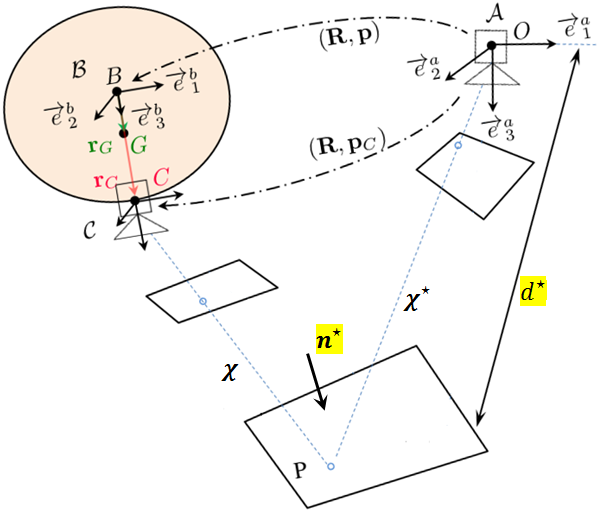
\includegraphics[width = 63mm]{Images/Notation_rot_modif3.png}
	\end{figure}\vspace{-0.5cm}
	$$\mathbf{\chi}^\star = \mathbf{p}_c + \mathbf{R}\mathbf{\chi} \Rightarrow \mathbf{\chi} = \mathbf{H}\mathbf{\chi}^\star$$ \vspace{-0.8cm}	
	
	\column[content...]{0.5\textwidth}
%	\begin{block}{Pose decomposition}
%		\begin{itemize}
%			\item No need!
%		\end{itemize}
%	\end{block}
	\pause
	\begin{block}{Homography}
		\vspace{-0.3cm}
		\begin{equation*}
		\mathbf{H} \triangleq \mathbf{R}^{\!\top} - \frac{1}{d^\star} \mathbf{R}^{\!\top} \mathbf{p}_C \mathbf{n}^{\star\!\top} 
		%\vspace{10cm}
		\end{equation*}
		\centering
		%$\mathbf{H}$ estimated from corresponding images
		%
	\end{block}	
	
\end{columns}
\end{frame}

\begin{frame}{Homography-based visual control}
\begin{columns}
	\column[content...]{0.6\textwidth}
	\begin{figure}
		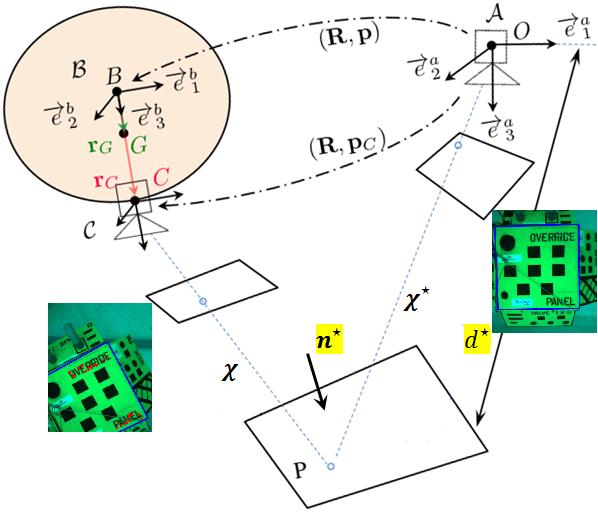
\includegraphics[width = 63mm]{Images/Notation_rot_modif4.png}
	\end{figure}\vspace{-0.5cm}
	$$\mathbf{\chi}^\star = \mathbf{p}_c + \mathbf{R}\mathbf{\chi} \Rightarrow \mathbf{\chi} = \mathbf{H}\mathbf{\chi}^\star$$ \vspace{-0.8cm}	
	
	\column[content...]{0.5\textwidth}
	%	\begin{block}{Pose decomposition}
	%		\begin{itemize}
	%			\item No need!
	%		\end{itemize}
	%	\end{block}
	
	\begin{block}{Homography}
		\vspace{-0.3cm}
		\begin{equation*}
		\mathbf{H} \triangleq \mathbf{R}^{\!\top} - \frac{1}{d^\star} \mathbf{R}^{\!\top} \mathbf{p}_C \mathbf{n}^{\star\!\top} 
		\end{equation*}
		\centering
		%$\mathbf{H}$ estimated from corresponding images
	\end{block}
	
	%	\begin{block}{Homography estimation}
	%		\begin{itemize}
	%			\item without any assumptions on the camera pose
	%			\item up to an unknown scalar factor
	%		\end{itemize}
	%	\end{block}
	%\pause
	\begin{exampleblock}{Measurements:}
		\begin{itemize}
			\item $\mathbf{H}$ {\footnotesize is estimated from corresponding images}
			\item $\mathbf{\Omega}, \mathbf{R}^\top \mathbf{e}_3 $ {\footnotesize are measured by IMU}
		\end{itemize}
	\end{exampleblock}
	\pause
	\begin{exampleblock}{Control objective}\vspace{-0.0cm}
		\[
		\begin{array}{rl}
		(\mathbf{R}, \mathbf{p}_c) & \longrightarrow (\mathbf{I}_3, \mathbf{0})\\
		\mathbf{H} & \longrightarrow \mathbf{I}_3\\
		%(\mathbf{e}_p, \mathbf{e}_\Theta) & \longrightarrow (\mathbf{0}, \mathbf{0})
		\end{array}
		\]	
	\end{exampleblock}
	
\end{columns}

\end{frame}

\begin{frame}{Kinematic control, recalled}
	%\begin{block}{S.Benhimane and E.Malis, 2007}
	%	Homography-based 2D visual tracking and servoing
	%\end{block}
	\begin{columns}
		\column[placement]{0.55\textwidth}
		\begin{block}{Lemma 1}
			%{\color{blue}{\scriptsize Source: Homography-based 2D visual tracking and servoing, \textbf{S.Benhimane and E.Malis}, \textit{Int. J. of Robotics Research}, 2007}} \\
			[{\color{blue}S.Benhimane et E.Malis, 2007}]
			\vspace{0.2cm}
%			Define visual errors:\vspace{-0.2cm}
%			\[
%			\begin{array}{rl}
%			\mathbf{e}_p &\triangleq (\mathbf{I}_3 - \mathbf{H})\mathbf{m}^\star\\
%			\mathbf{e}_\Theta &\triangleq \mathrm{vex}(\mathbf{H}^\top - \mathbf{H}) 
%			\end{array}
%			\]	
			
			The \textbf{kinematic} control law
			\vspace{-0.2cm}			
			\begin{equation*}\label{maliscontrol}
			\mathbf{V}_{C} = -k_p \mathbf{e}_p\,,\quad \mathbf{\Omega} = -k_\Theta \mathbf{e}_\Theta 
			\vspace{-0.2cm} 
			\end{equation*}
			with $k_p, k_\Theta>0$, 
			ensures the local exponential stability of $\mathbf{H}  \rightarrow \mathbf{I}_3$. 
			\\
			\vspace{0.3cm}
			\centering
			$[\mathbf{e}_p^\top, \mathbf{e}_\Theta^\top]^\top = \mathbf{0} \Leftrightarrow \mathbf{H} = \mathbf{I}_3$ 
		\end{block}
		\column[placement]{0.45\textwidth}
		\vspace{-0.5cm}
		\begin{block}{Visual errors}
			\vspace{-0.5cm}
			\[
			\begin{array}{rl}
			\mathbf{e}_p &\triangleq (\mathbf{I}_3 - \mathbf{H})\mathbf{m}^\star\\
			\mathbf{e}_\Theta &\triangleq \mathrm{vex}(\mathbf{H}^\top - \mathbf{H}) 
			\end{array}	\vspace{-0.3cm}	
			\]
			\centering
			with $\mathbf{m}^\star \in S^2$ satisfying: \vspace{-0.4cm}
			\[
			\begin{array}{ll} 
			%|\mathbf{m}^\star| &= 1 \\
			\mathbf{n}^{\star \top} \mathbf{m}^\star &> 0
			\end{array}
			\]		
		\end{block}\vspace{-0.2cm}
		\pause
		\begin{block}{Advantage}
			\begin{itemize}
				\item No need of homography decomposition				
			\end{itemize}
		\end{block}\vspace{-0.2cm}
		\pause
		\begin{exampleblock}{\small Passage to dynamic control} 
			\begin{itemize}
				\item Require $\dot{\mathbf{V}}_{Cr} $ and $\dot{\mathbf{\Omega}}_{r} $ 
				\item \textbf{Unknown} $\mathbf{n}^{\star}$ and $d^\star$ \\
				$\Rightarrow$ {\color{red} $\dot{\mathbf{e}}_p, \dot{\mathbf{e}}_\Theta$ not calculable}\\	
				$\!\!\!\!\!\!\!\Rightarrow$ $\dot{\mathbf{V}}_{Cr} $  $\dot{\mathbf{\Omega}}_{r}$ not calculable			
			\end{itemize}
		\end{exampleblock}
	\end{columns}
\end{frame}

\begin{frame}{Outer loop control design}
%Block diagram of the proposed HBVS controller
\begin{figure}
	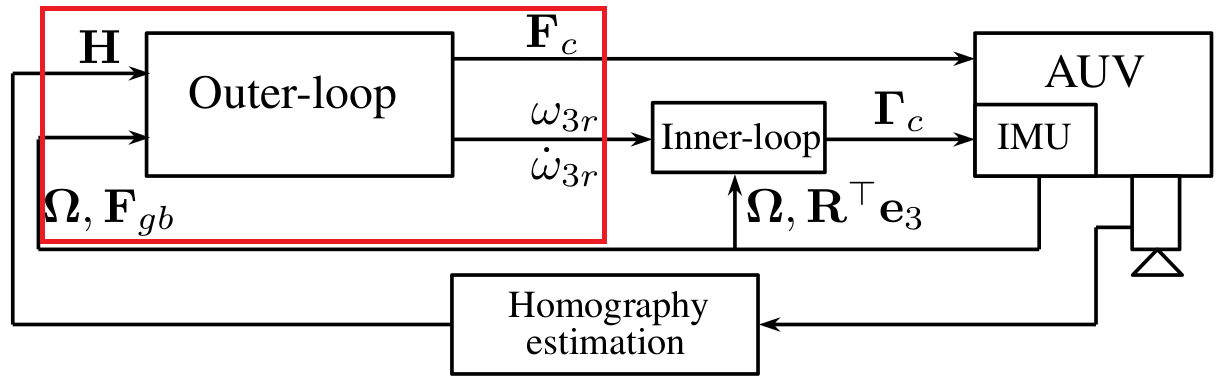
\includegraphics[width = 90mm]{Images/Block_diagram_2_outer.png}
\end{figure}
\begin{itemize}
	%\item \textbf{Inner loop}:
	%\begin{itemize}		
	%	\item $\mathbf{\Gamma}_C$ ensures  
	%	$(\mathbf{\Omega}, \mathbf{R}^\top \mathbf{e}_3) \rightarrow (\mathbf{\Omega}_r, \mathbf{e}_3)$\\
		%where: $ \mathbf{\Omega}_r \stackrel{\triangle}{=}  k_g \mathbf{e}_3 \times \mathbf{R}^{T} \mathbf{e}_3 + \omega_{3r} \mathbf{e}_3$ 
	%\end{itemize} 	
	\item \textbf{Outer loop}:
	\begin{itemize}
		\item $\mathbf{F}_c$ ensures $(\mathbf{e}_p, \mathbf{V}) \rightarrow (\mathbf{0},\mathbf{0})$
		\item $\mathbf{F}_c$ combined with $\mathbf{\Omega}_{r}$ ensure $\mathbf{H} \rightarrow \mathbf{I}_3$		
	\end{itemize}
\end{itemize}
\end{frame}

\begin{frame}{Outer-loop control force $\mathbf{F}_c$ design: {\bf \color{red} Control design principle}}
	\begin{itemize}
		\item \textbf{Basic system}: 
		\begin{equation*}
		\left\{
		\begin{array}{ll}
		\dot {{e}}_p &\!\!\!\!= {\color{red} a^\star} V \\
		\dot{{V}}&\!\!\!\!=  u
		\end{array}\right. \vspace{-0.15cm}
		\end{equation*}\\
		where: $e_p, a^\star, V \in \mathbb{R};{\color{red} \quad \text{unknown}\; a^\star    >0}; \quad u \; \text{control input}$
		\pause
		\vspace{1cm}
		\item  If $V$ is \textbf{measured}, define \textbf{control law} 
		$$u = - k_1 e_p - k_2 V; {\quad \; k_1, k_2>0}$$
		
		$\Rightarrow$ Stable second order system: $\ddot{e}_p + k_2 \dot{e}_p + a^\star k_1 e_p = 0$	
	\end{itemize}
\end{frame}

\begin{frame}{Outer-loop control force $\mathbf{F}_c$ design: {\bf \color{red} Control design principle}}
\begin{itemize}
	\item \textbf{Basic system}: 
	\begin{equation*}
	\left\{
	\begin{array}{ll}
	\dot {{e}}_p &\!\!\!\!= {\color{red} a^\star} V \\
	\dot{{V}}&\!\!\!\!=  u
	\end{array}\right. \vspace{-0.15cm}
	\end{equation*}\\
	where: $e_p, a^\star, V \in \mathbb{R};{\color{red} \quad \text{unknown}\; a^\star    >0}; \quad u \; \text{control input}$
	\vspace{1cm}
	\item If $V$ is \textbf{{\color{red} not}  measured}. 
	\pause
	Introduce:
	\begin{itemize}
		\item  {\color{red}\textbf{augmented system}: $\dot{\hat{e}}_p = - k_1(\hat{e}_p - e_p);$} $\quad  k_1 >0$
		\item \textbf{control law}: $u = k_2(\hat{e}_p - e_p) - k_3 e_p; \quad k_2, k_3 >0 $ 
	\end{itemize}
	\pause
	Lyapunov function: 
	$\mathcal{L} = \dfrac{1}{2} (\hat{e}_p - e_p)^2 + \dfrac{k_3}{2k_2} e^2_p + \dfrac{a^\star}{2k_2} V^2
	$ \\
	$\Rightarrow \dot{\mathcal{L}} = -k_1 (\hat{e}_p - e_p)^2 \le 0$\\
	$\Rightarrow \hat{e}_p \rightarrow e_p; V \rightarrow 0; e_p \rightarrow 0$		
\end{itemize}
\end{frame}



%\begin{frame}{Outer-loop control design, $\mathbf{F}_c$}
%	\begin{block}{Proposition 1, $\mathbf{v}_f = \mathbf{0}$}
%		\begin{itemize}
%			\item There exist: \\
%			\begin{itemize}
%				\item $\dot {\mathbf{e}}_p = -\mathbf{\Omega}\times  \mathbf{e}_p   + \frac{(\mathbf{n}^{\star\top}\mathbf{m}^\star)}{d^\star} \mathbf{V} + \boldsymbol{\varepsilon}(t), \boldsymbol{\varepsilon}(t) \text{ bounded and}  \longrightarrow 0$
%				\item 
%				$\mathbf{M}\dot{\mathbf{V}} = (\mathbf{M}\mathbf{V}) \!\times\!\mathbf{\Omega} + \mathbf{F}_c + \mathbf{F}_{gb} + \mathbf{F}_d(\mathbf{V}), \mathbf{\Delta}_F = 0 $ 
%			\end{itemize}
%			\item Introduce: \\
%			\begin{itemize}
%				\item $\dot {\hat{\mathbf{e}}}_p = -\mathbf{\Omega}\times  \hat{\mathbf{e}}_p   -\mathbf{K}_1 \hat{\mathbf{e}}_p + \mathbf{K}_1 {\mathbf{e}}_p, \quad  \hat{\mathbf{e}}_p(0) \in \mathbb{R}^3$
%				\item
%%				$\mathbf{F}_c \!=\! \bar m \mathbf{M}^{-1} \big(\mathrm{sat}^{\eta_1}(k_2 \tilde{\mathbf{e}}_p)  - \mathrm{sat}^{\eta_2}( k_3 {\mathbf{e}}_p) \big) - \mathbf{F}_{gb}$ 
%				$\mathbf{F}_c \!=\! \bar m \mathbf{M}^{-1} \big(k_2(\hat{\mathbf{e}}_p - \mathbf{e}_p)  -  k_3 {\mathbf{e}}_p \big) - \mathbf{F}_{gb}$ 
%			\end{itemize}
%			\item Conclusion:\\ $(\mathbf{e}_p,{\hat{\mathbf{e}}}_p, \mathbf{V})=(\mathbf{0},\mathbf{0},\mathbf{0})$  globally asymptotically stable (GAS)			 
%		\end{itemize}		
%	\end{block}	
%\end{frame}

%\begin{frame}{Outer-loop control design, $\omega_{3r}$}
%	\begin{block}{Proposition 3, $\mathbf{v}_f = \mathbf{0}$:}
%		\begin{itemize}
%			\item If:
%			\begin{itemize}
%				\item $\mathbf{\Gamma}_c$ ensures almost-GAS of the equilibrium $(\mathbf{\Omega}, \mathbf{R}^\top \mathbf{e}_3) = (\mathbf{\Omega}_r, \mathbf{e}_3)$, with $\mathbf{\Omega}_r$ defined by $$\mathbf{\Omega}_r \triangleq k_g \mathbf{e}_3 \times \mathbf{R}^\top \mathbf{e}_3 + \omega_{3r} \mathbf{e}_3, k_g >0  $$
%				$$\dot{\omega}_{3r} = -k_{\Theta 2} \omega_{3r} - k_{\Theta 1} \mathrm{sat}^{\Delta_\Theta}(h_{1,2})$$
%				 $$\quad \omega_{3r}(0) \in \mathbb{R}; k_{\Theta 1}, k_{\Theta 2}, \Delta_\Theta> 0$$
%				\item $\mathbf{F}_c$ given by Proposition 1
%			\end{itemize}
%			\item Then: $\mathbf{H} = \mathbf{I}_3$ is almost-GAS.
%		\end{itemize}
%	\end{block}	
%\end{frame}

\begin{frame}{Outer-loop $\Omega_{r}$ design: basic idea}
\begin{block}{Control objective}
	\centering
	$(\mathbf{e}_p, \mathbf{e}_\Theta) \rightarrow (\mathbf{0}, \mathbf{0})$
\end{block}
\begin{block}{$\Omega_{r}$ design:}
	\begin{itemize}
		\item \small Defined $\mathbf{F}_c \Rightarrow  \mathbf{e}_p = \mathbf{0}$ 
		\pause
		\item Inner-loop $\mathbf{\Gamma}_c \Rightarrow$  $(\mathbf{\Omega}, \mathbf{R}^\top \mathbf{e}_3) = (\mathbf{\Omega}_r, \mathbf{e}_3)$ \\
		\begin{itemize}
			\pause
			\item $\mathbf{R}^\top \mathbf{e}_3 \rightarrow \mathbf{e}_3 \Rightarrow $ roll and pitch angles are stabilized to zero	\vspace{-0.2cm}		 		
			\pause	
			\begin{equation*}	\vspace{-1.4cm}		
			\left.\begin{aligned}			
			\mathbf{e}_p & \rightarrow \mathbf{0}  \\
			\mathbf{R}^\top \mathbf{e}_3 & \rightarrow  \mathbf{e}_3
			\end{aligned}
			\right\}
			\text{$\; \Rightarrow h_{1,2} \rightarrow \sin \psi + \kappa (1-\cos \psi); \; \kappa = const >0$}
			%$\Rightarrow h_{1,2} \longrightarrow $
			\end{equation*}
			\item 
		\end{itemize}
	    \vspace{0.7cm}
	    \pause
		\item To stabilize $h_{1,2} \rightarrow 0$, ( $\Rightarrow \psi \rightarrow 0$, $(\mathbf{p}_c, \mathbf{R}) \rightarrow (\mathbf{0}, \mathbf{I}_3)$) : %\vspace{-0.8cm}		
		
		${\color{red} \dot{\omega}_{3r} = -k_{\Theta 2} \omega_{3r} - k_{\Theta 1}h_{1,2}}, \; {\quad  \omega_{3r}(0) \in \mathbb{R}; k_{\Theta 1}, k_{\Theta 2}> 0}$\\
		%\vspace{-0.7cm}
		%\pause
		${\color{red} \mathbf{\Omega}_r \triangleq k_g \mathbf{e}_3 \times \mathbf{R}^\top \mathbf{e}_3 + \omega_{3r} \mathbf{e}_3}, \quad k_g >0  $ \\	
	\vspace{0.1cm}				
	{\tiny(\color{blue} \textbf{See more}: An inertial-aided homography-based visual servoing control approach for (almost) fully-actuated AUVs, \textbf{S.Krupinski, G.Allibert, M.-D. Hua, T. Hamel}, \textit{IEEE Transactions on robotics}, 2017).}
	\end{itemize}
\end{block}	
\end{frame}




\begin{frame}{Inner-loop control design}
	%Since the rotation dynamics is fully-actuated and both $\mathbf{\Omega}$ and $\mathbf{R}^\top \mathbf{e}_3$ are measured, it is not too difficult to design an effective inner-loop torque control that ensures  $(\mathbf{\Omega}, \mathbf{R}^\top \mathbf{e}_3) \longrightarrow (\mathbf{\Omega}_r, \mathbf{e}_3)$
	
	\begin{figure}
		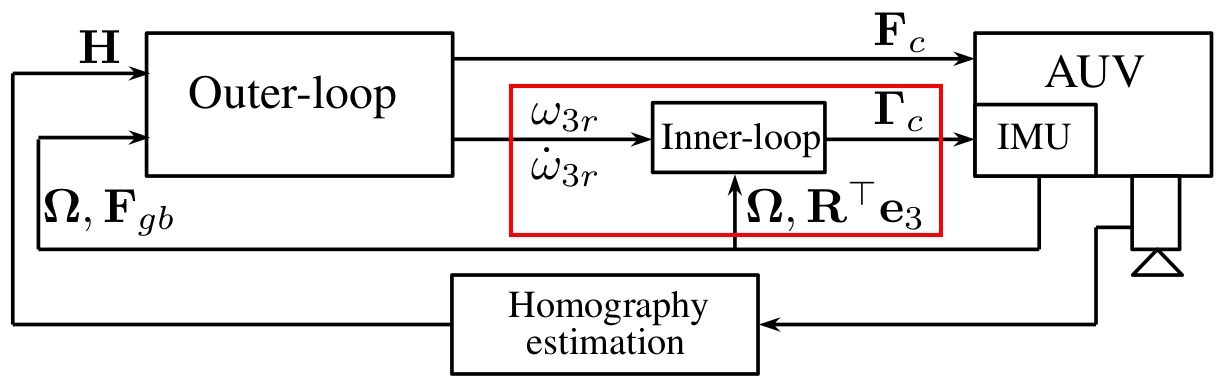
\includegraphics[width=90mm]{Images/Block_diagram_2_inner.png}
	\end{figure}
	
	\begin{itemize}
		\item \textbf{Fully-actuated} rotation dynamics
		\item Both $\mathbf{\Omega}$ and $\mathbf{R}^\top \mathbf{e}_3$ are \textbf{measured} \\
		$\Rightarrow$ {\color{red} \textbf{Not}} too difficult to design $\mathbf{\Gamma}_c$ ensuring $(\mathbf{\Omega}, \mathbf{R}^\top \mathbf{e}_3) \rightarrow (\mathbf{\Omega}_r, \mathbf{e}_3)$ 
	\end{itemize}
\end{frame}

\begin{frame}{Enhanced controller}
%Practical issues:\\
%- Imprecise model parameters\\
%- Current leads to "Munk moment" cannot be ignored\\
%requires that control laws must be robust  <- integral action\\
%Need to estimate disturbance $\mathbf{\Delta}_{\Gamma}$

	\begin{itemize}
		\item \textbf{Practical issues}: \\
		- Imprecise model parameters\\
		- "Munk moment" cannot be ignored due to current $\mathbf{v}_f \neq \mathbf{0}$
		\vspace{0.5cm}
		\item \textbf{Controller enhanced} by adding:\\
		- \textbf{\color{red} Integrators} in both inner and outer loops\\
		  %$\; \; \Rightarrow $  Only {\color{red} local exponential stability}  \\
		- \textbf{\color{red} Estimator} of disturbance $\mathbf{\Delta}_{\Gamma}$		
	\end{itemize}
 
\end{frame}

\section{Simulation results}
\begin{frame}{Simulation results, \tiny$\mathbf{p}_C(0) = [-2, -1.5, -1 ]^{\top} (m)$, $\mathbf{R}(0) = \mathbf{R}_{\{\frac{\pi}{18},-\frac{\pi}{18},\pi\}}$, $\mathbf{V}(0) = \mathbf{\Omega}(0) = \mathbf{0}$}

\begin{block}{Current $\mathbf{V}_f = \mathbf{0}$}
	\begin{figure}
		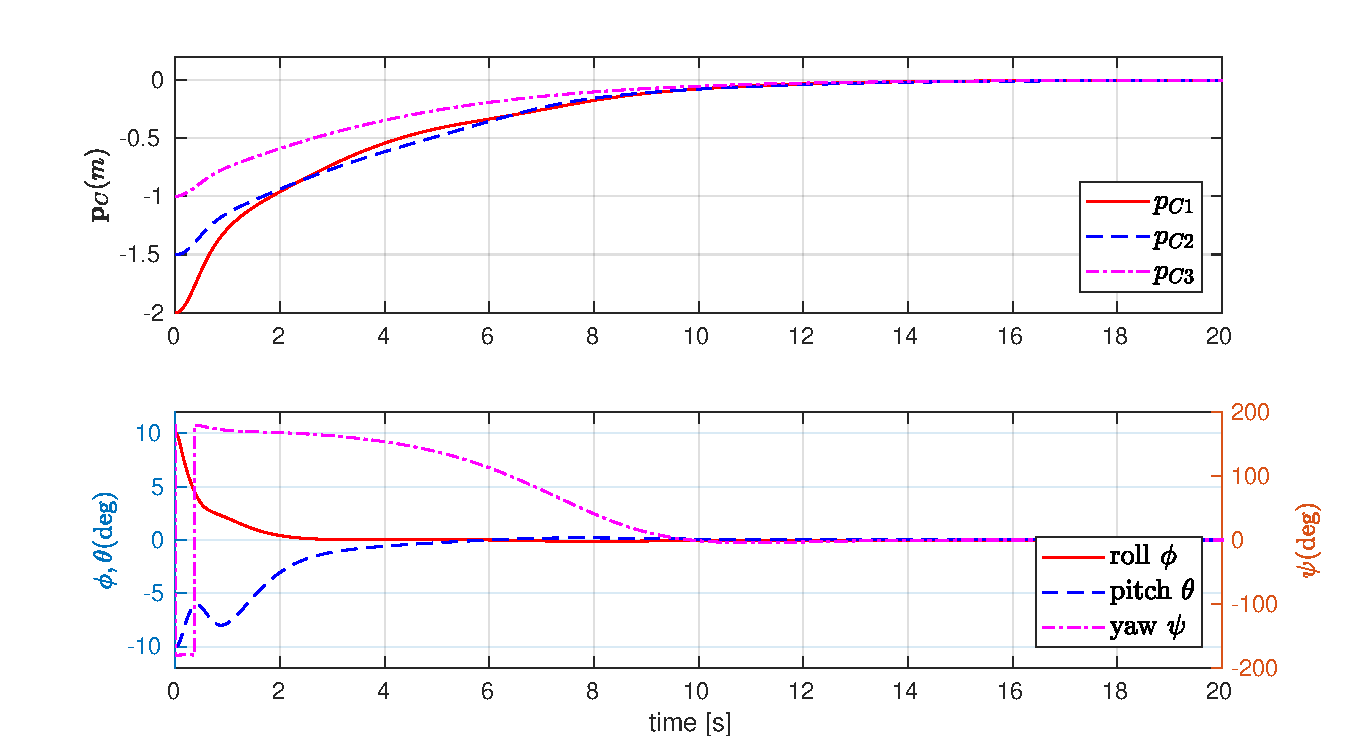
\includegraphics[width = 105mm]{Images/Data_sansCurrent_pos_RollPitch_Yaw2.pdf}
	\end{figure}
\end{block}
\end{frame}

\begin{frame}{Simulation results, \tiny$\mathbf{p}_C(0) = [-2, -1.5, -1 ]^{\top} (m)$, $\mathbf{R}(0) = \mathbf{R}_{\{\frac{\pi}{18},-\frac{\pi}{18},\pi\}}$, $\mathbf{V}(0) = \mathbf{\Omega}(0) = \mathbf{0}$}

\begin{block}{Current $\mathbf{V}_f = [\dfrac{1}{2\sqrt{2}}, \dfrac{1}{2\sqrt{2}}, 0] (m/s)$}
	\begin{figure}
		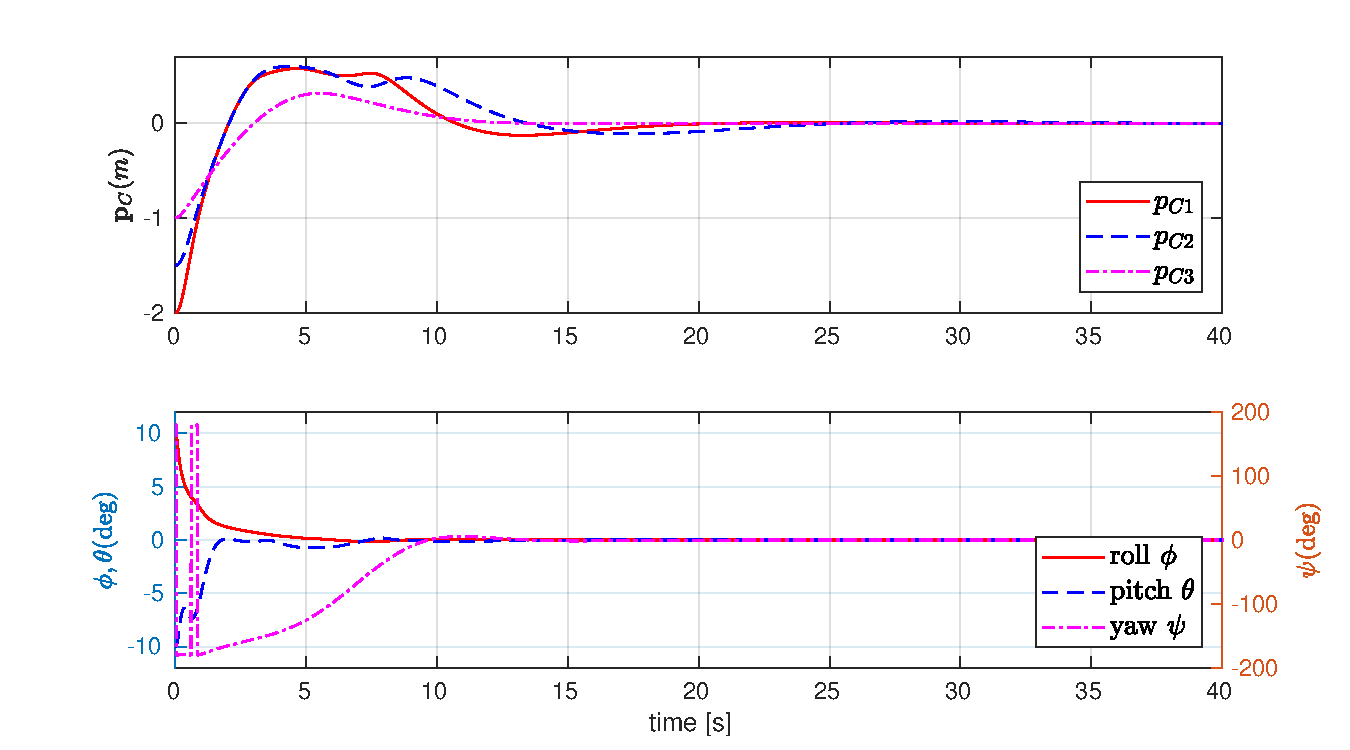
\includegraphics[width = 105mm]{Images/Data_avecCurrent_pos_RollPitch_Yaw2.pdf}	
	\end{figure}
\end{block}
\end{frame}

\section{Conclusion}

\begin{frame}{Conclusion}

  % Keep the summary *very short*.
  A new \textbf{inertial-aided homography-based visual servo} controller was proposed for the stabilisation of \textbf{compact fully-actuated} AUVs:
  \begin{itemize}
  \footnotesize
  \item
    %The \alert{first main message} of your talk in one or two lines.
    By using image-based \textbf{homography without its decomposition}.
  \item
    \textbf{Without relying on linear velocity measurement ({\color{red}no need DVL})}
 % \item
 %   It ensures \textbf{locally exponential stability}, with \textbf{robustness} to unmodeled dynamics and disturbance.
  \end{itemize}
\vspace{0.5cm}

\begin{columns}
	\column[content...]{0.38\textwidth}
	\begin{block}{DVL}
		\begin{figure}
			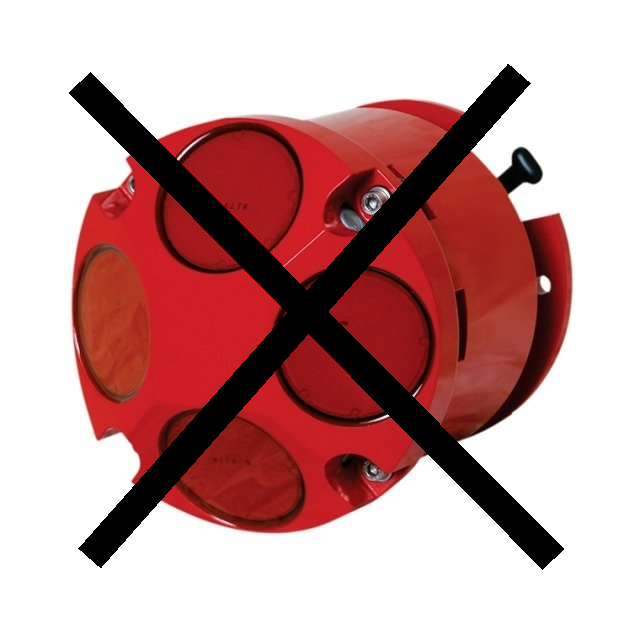
\includegraphics[width = 0.65\textwidth]{Images/DVL_no.png}\\
			\tiny {\color{blue} Source: www.teledyne.com}
		\end{figure}
	\end{block}
	\pause
	\column[content...]{0.64\textwidth}
		\begin{block}{Testbed}
		\begin{figure}
			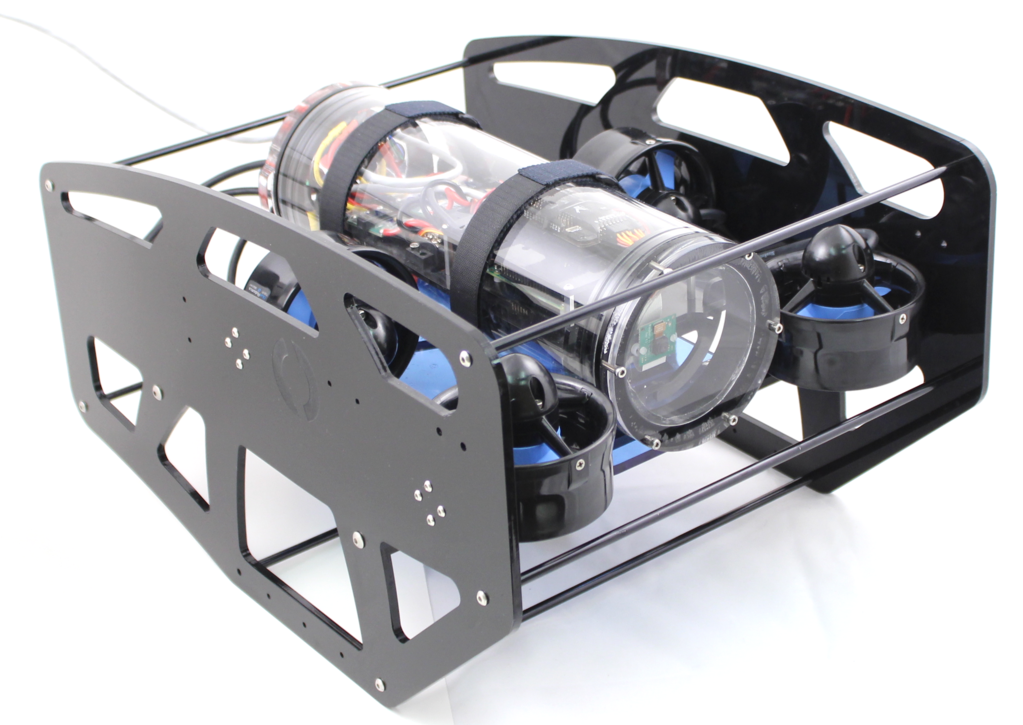
\includegraphics[width = 0.6\textwidth]{Images/Bluerov_modif.png}
			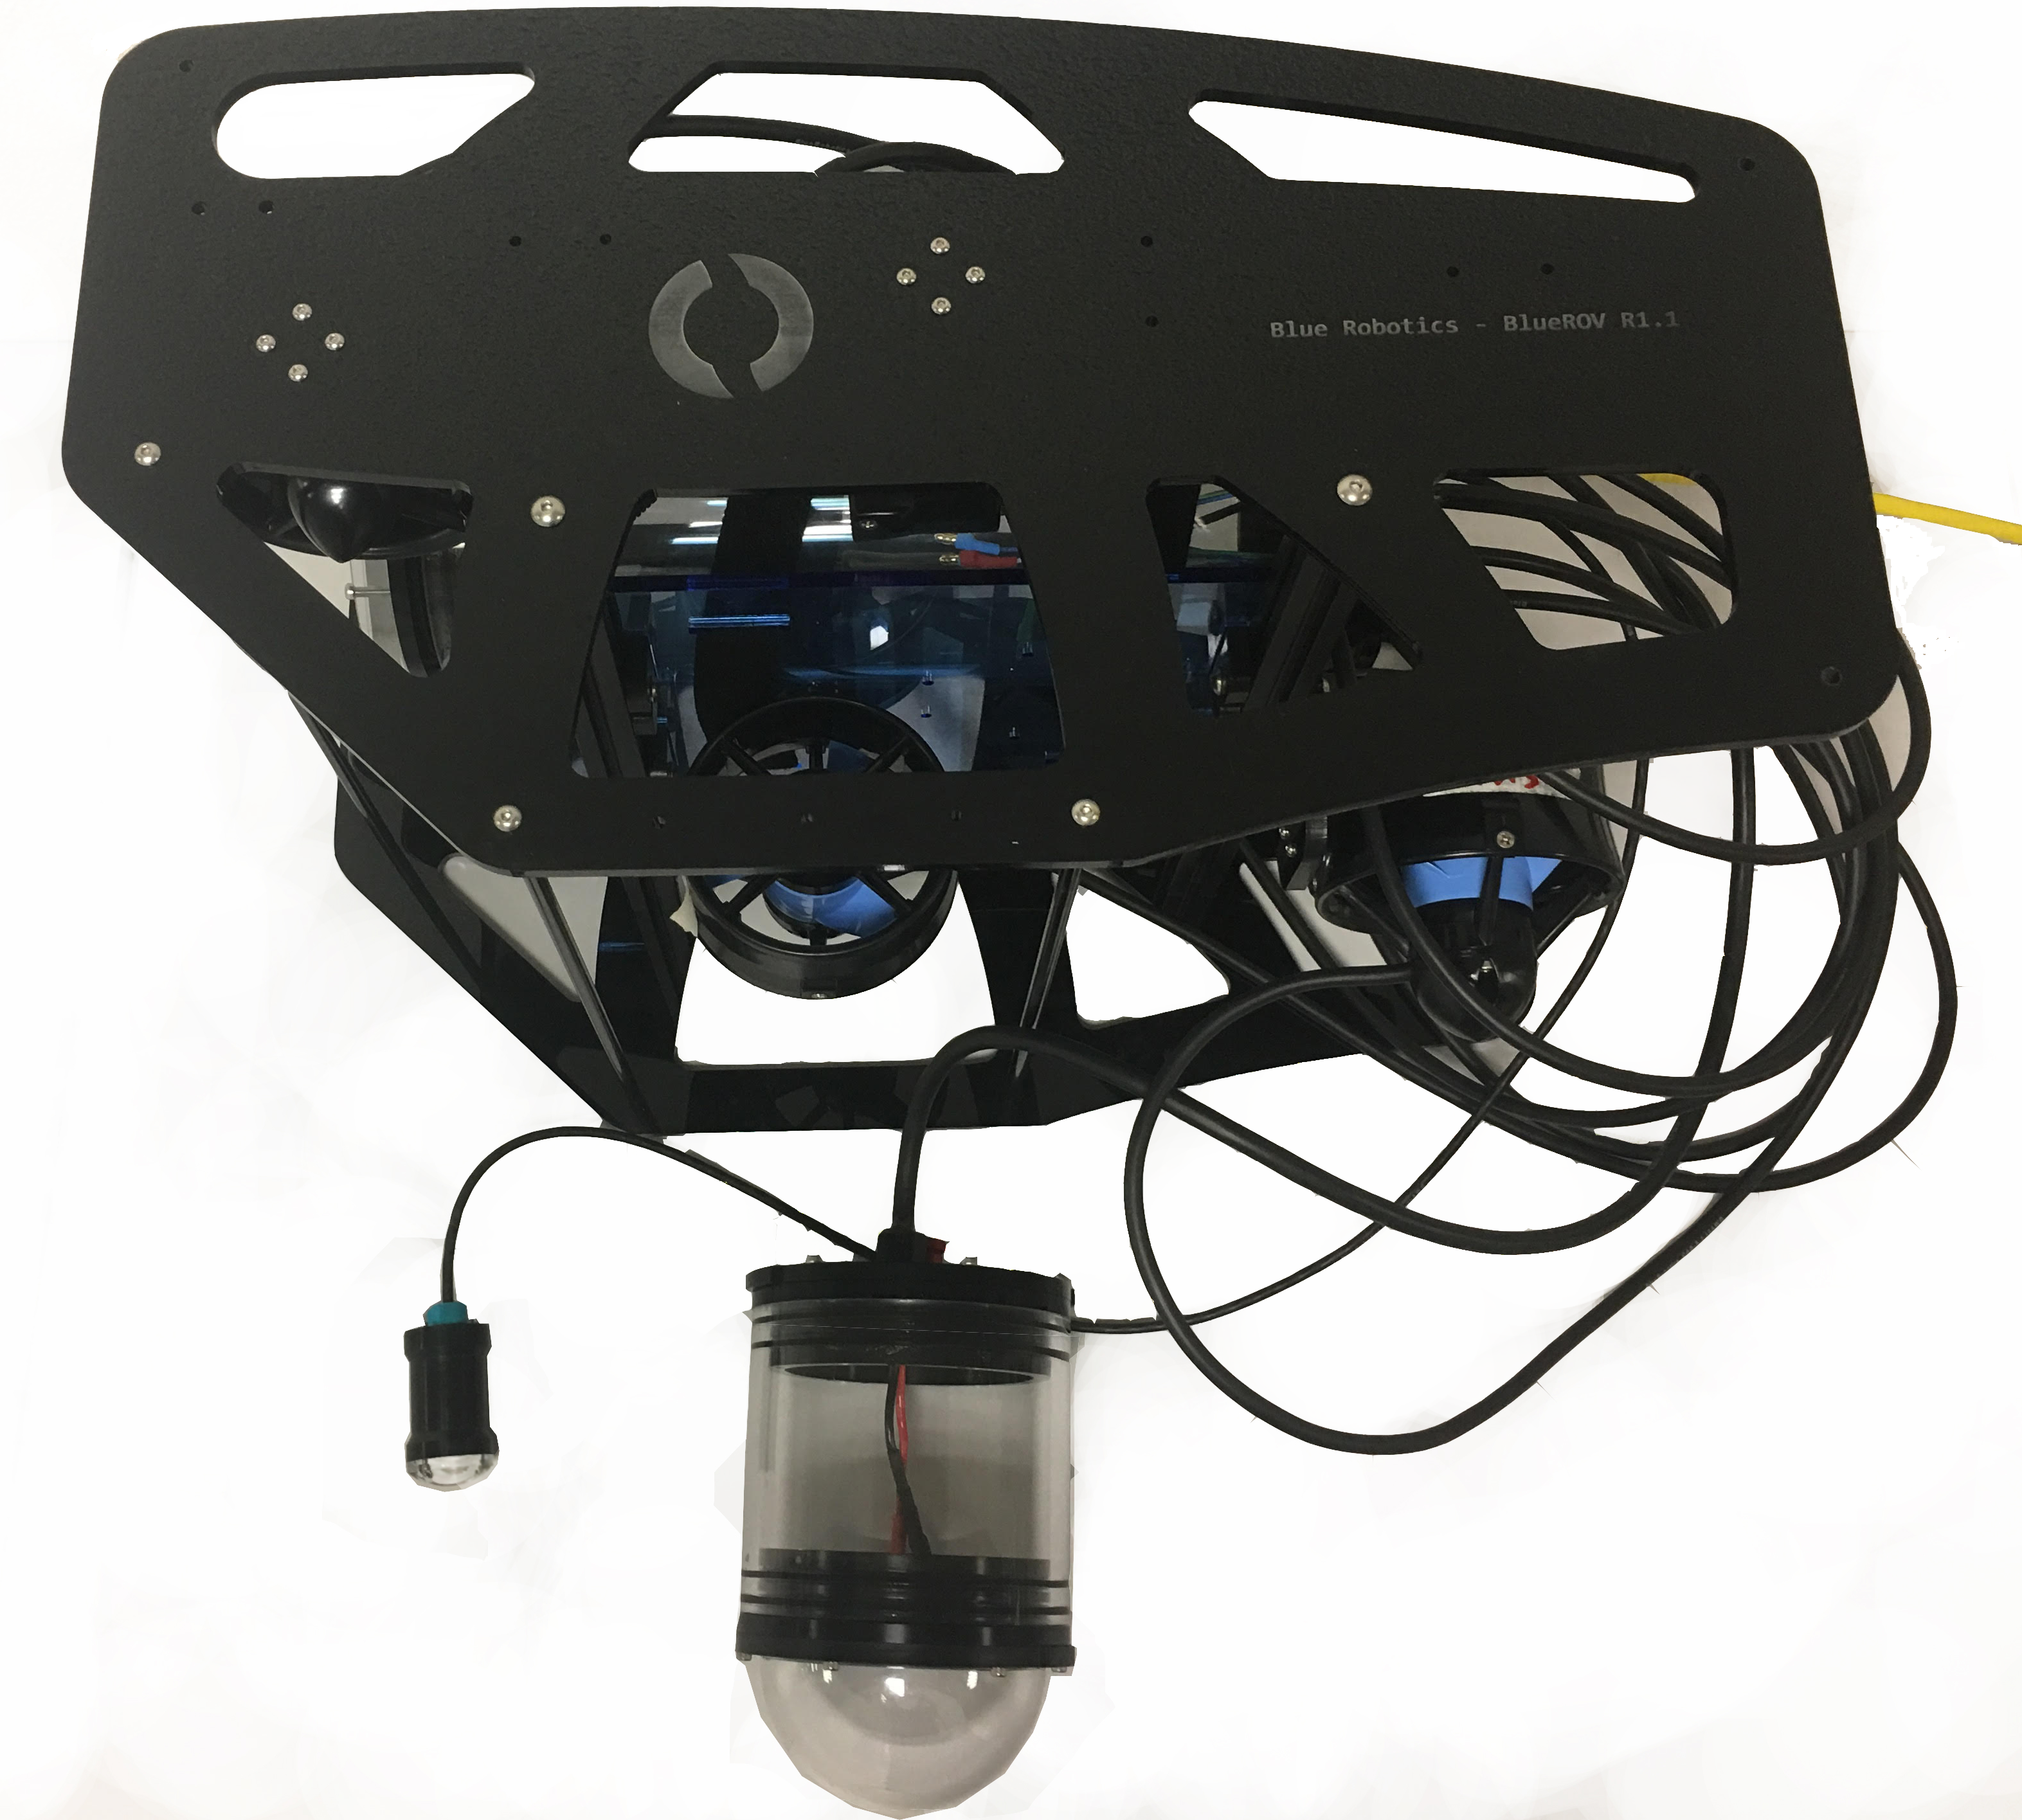
\includegraphics[width = 0.4\textwidth]{Images/I3S_UAV.png}
			%\tiny {\color{blue} Source: www.bluerobotics.com}
		\end{figure}
	\end{block}
	
	

	\end{columns}
  
  % The following outlook is optional.
  \vskip0pt plus.5fill

\end{frame}


\begin{frame}
\centering {
	{\huge \textbf{Thank you for your attention!}}	
	{\huge \textbf{Q\&A}}}


\end{frame}


\begin{frame}{Simulation results, \tiny$\mathbf{p}_C(0) = [-2, -1.5, -1 ]^{\top} (m)$, $\mathbf{R}(0) = \mathbf{R}_{\{\frac{\pi}{18},-\frac{\pi}{18},\pi\}}$, $\mathbf{V}(0) = \mathbf{\Omega}(0) = \mathbf{0}$}

\begin{block}{Current $\mathbf{V}_f = \mathbf{0}$}
	\begin{figure}
		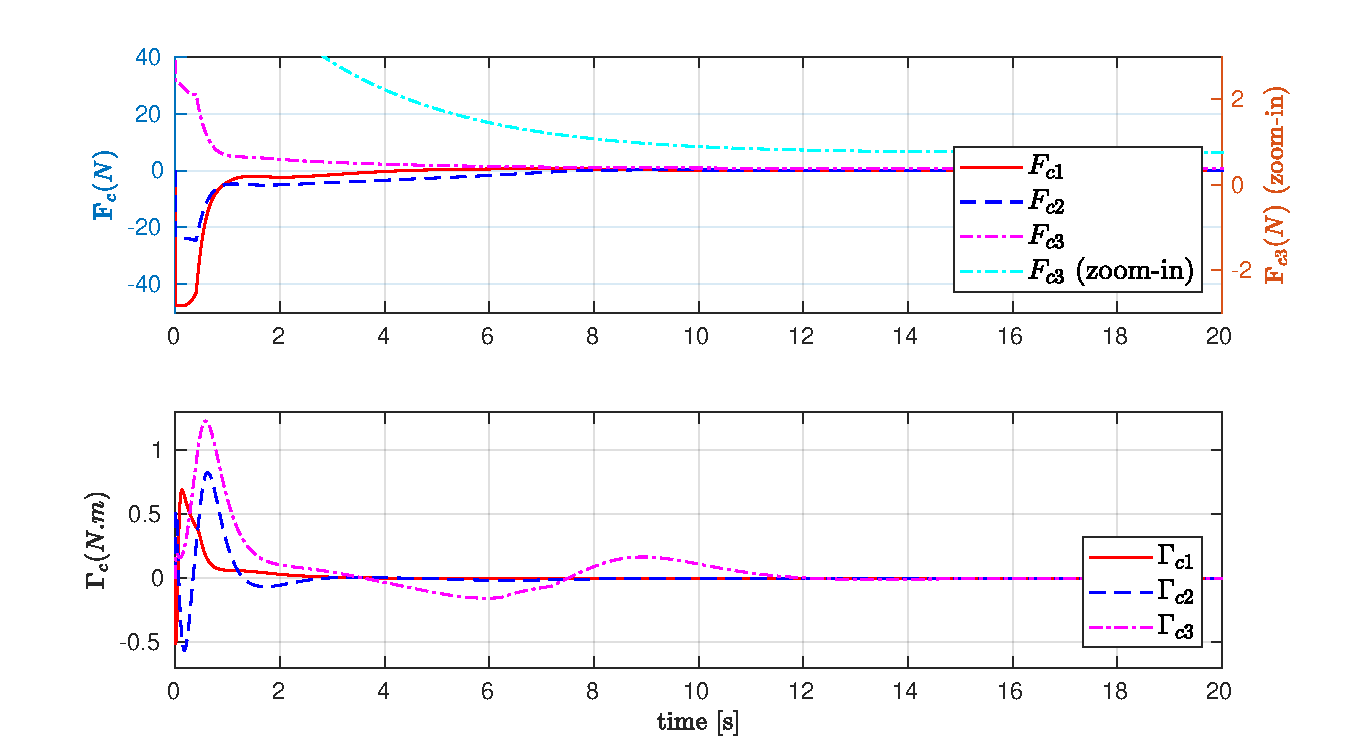
\includegraphics[width = 105mm]{Images/Data_sansCurrent_Fc_Gc2.pdf}
	\end{figure}
\end{block}
\end{frame}

\begin{frame}{Simulation results, \tiny$\mathbf{p}_C(0) = [-2, -1.5, -1 ]^{\top} (m)$, $\mathbf{R}(0) = \mathbf{R}_{\{\frac{\pi}{18},-\frac{\pi}{18},\pi\}}$, $\mathbf{V}(0) = \mathbf{\Omega}(0) = \mathbf{0}$}

\begin{block}{Current $\mathbf{V}_f = \mathbf{0}$}
	\begin{figure}
		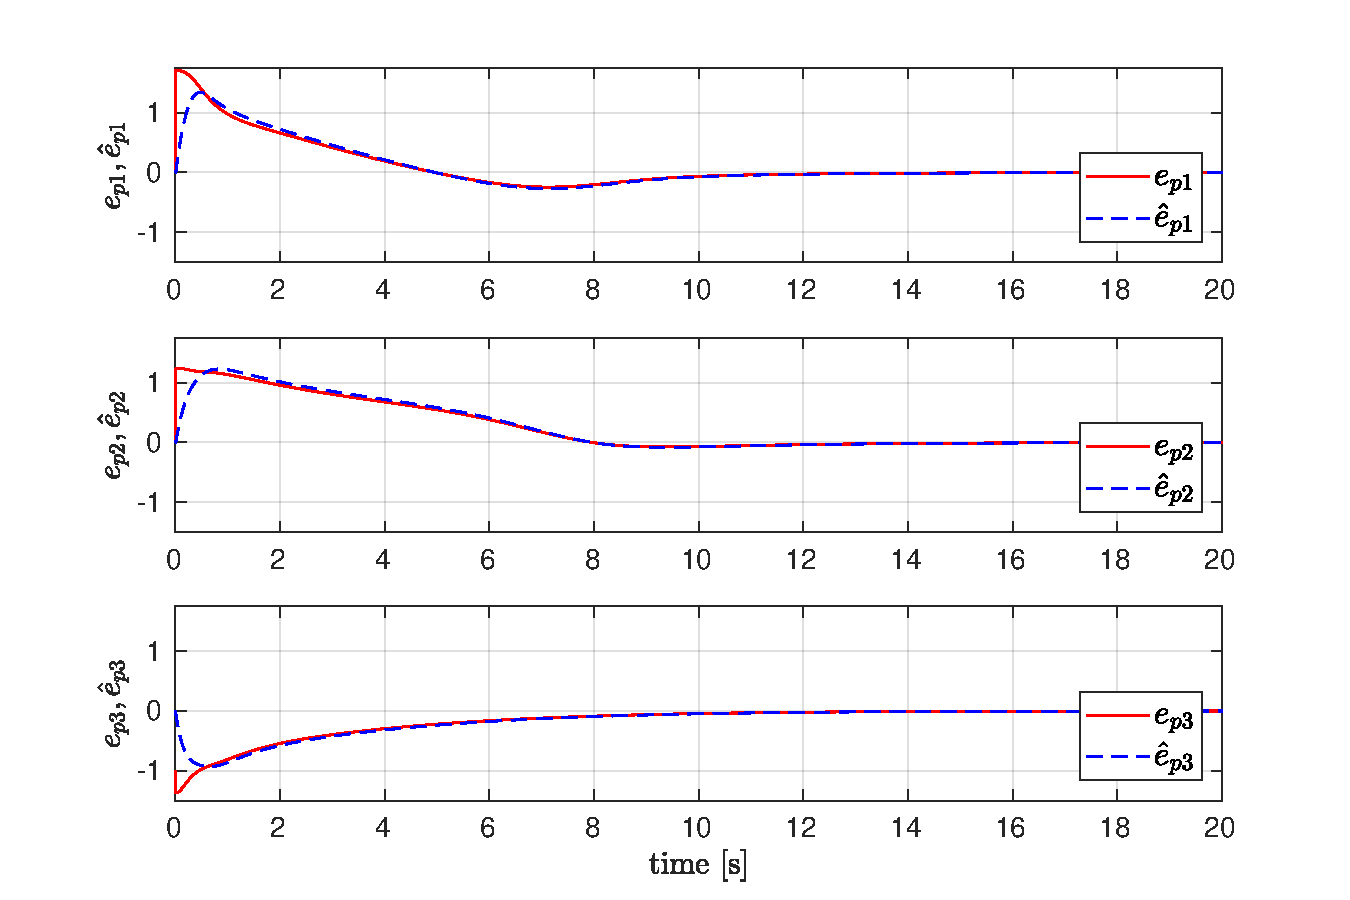
\includegraphics[width = 105mm]{Images/Data_sansCurrent_ep_epHat2.pdf}
	\end{figure}
\end{block}
\end{frame}

\begin{frame}{Simulation results, \tiny$\mathbf{p}_C(0) = [-2, -1.5, -1 ]^{\top} (m)$, $\mathbf{R}(0) = \mathbf{R}_{\{\frac{\pi}{18},-\frac{\pi}{18},\pi\}}$, $\mathbf{V}(0) = \mathbf{\Omega}(0) = \mathbf{0}$}

\begin{block}{Current $\mathbf{V}_f = \mathbf{0}$}
	\begin{figure}
		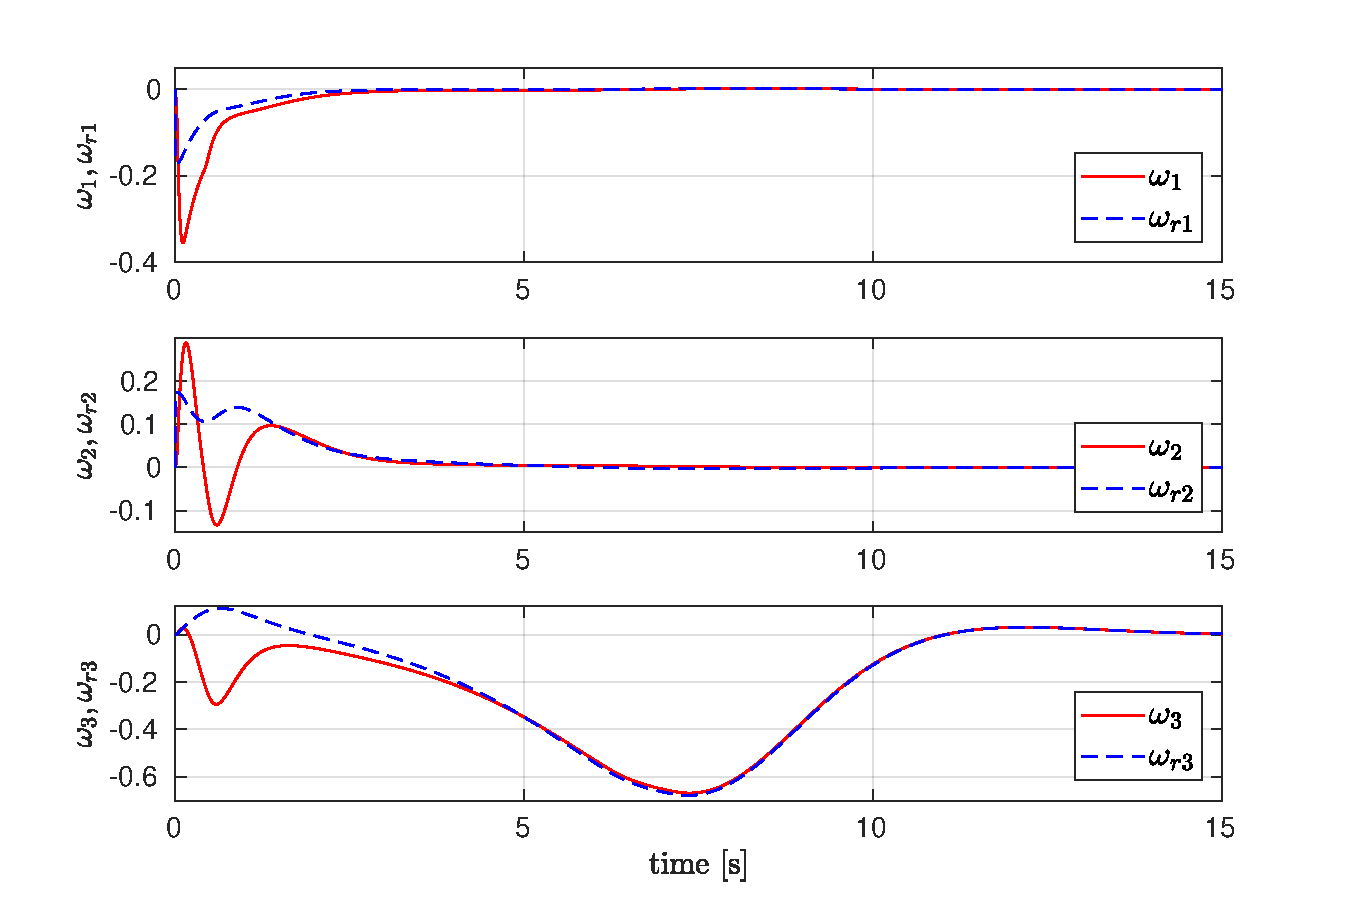
\includegraphics[width = 105mm]{Images/Data_sansCurrent_Om_Omr.pdf}
	\end{figure}
\end{block}
\end{frame}


\begin{frame}{Simulation results, \tiny$\mathbf{p}_C(0) = [-2, -1.5, -1 ]^{\top} (m)$, $\mathbf{R}(0) = \mathbf{R}_{\{\frac{\pi}{18},-\frac{\pi}{18},\pi\}}$, $\mathbf{V}(0) = \mathbf{\Omega}(0) = \mathbf{0}$}

\begin{block}{Current $\mathbf{V}_f = [\dfrac{1}{2\sqrt{2}}, \dfrac{1}{2\sqrt{2}}, 0] (m/s)$}
\begin{figure}
	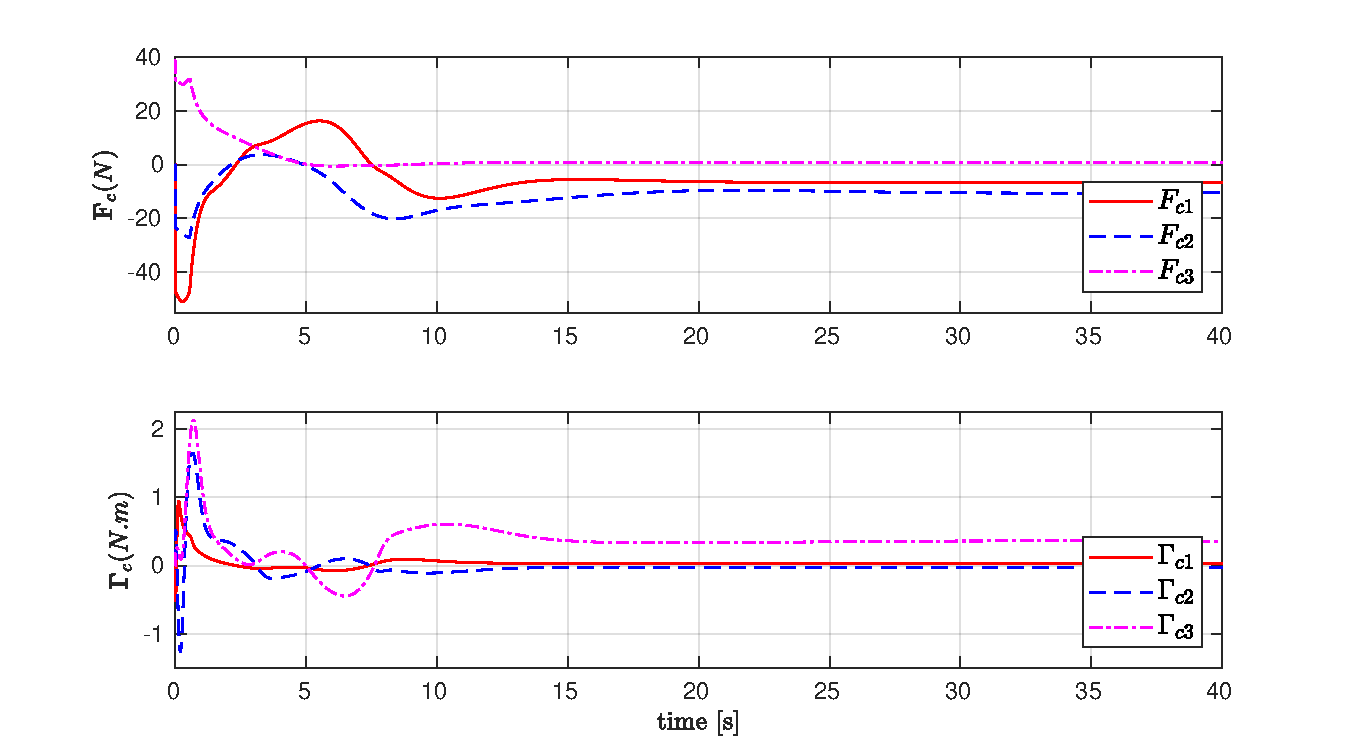
\includegraphics[width = 105mm]{Images/Data_avecCurrent_Fc_Gc2.pdf}	
\end{figure}
\end{block}
\end{frame}

\begin{frame}{Simulation results, \tiny$\mathbf{p}_C(0) = [-2, -1.5, -1 ]^{\top} (m)$, $\mathbf{R}(0) = \mathbf{R}_{\{\frac{\pi}{18},-\frac{\pi}{18},\pi\}}$, $\mathbf{V}(0) = \mathbf{\Omega}(0) = \mathbf{0}$}

\begin{block}{Current $\mathbf{V}_f = [\dfrac{1}{2\sqrt{2}}, \dfrac{1}{2\sqrt{2}}, 0] (m/s)$}
	\begin{figure}
		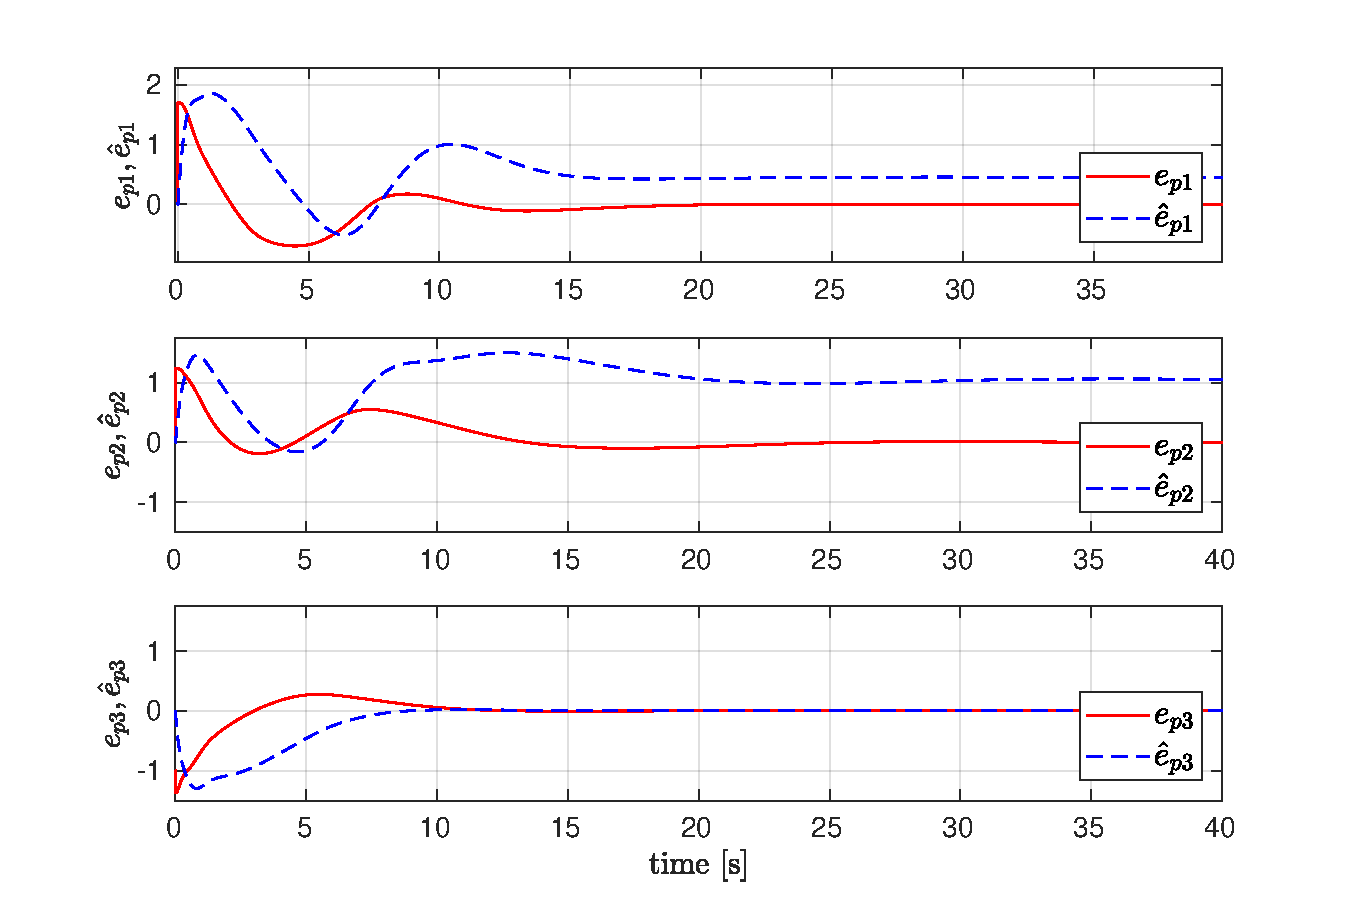
\includegraphics[width = 105mm]{Images/Data_avecCurrent_ep_epHat2.pdf}	
	\end{figure}
\end{block}
\end{frame}
\begin{frame}{Simulation results, \tiny$\mathbf{p}_C(0) = [-2, -1.5, -1 ]^{\top} (m)$, $\mathbf{R}(0) = \mathbf{R}_{\{\frac{\pi}{18},-\frac{\pi}{18},\pi\}}$, $\mathbf{V}(0) = \mathbf{\Omega}(0) = \mathbf{0}$}

\begin{block}{Current $\mathbf{V}_f = [\dfrac{1}{2\sqrt{2}}, \dfrac{1}{2\sqrt{2}}, 0] (m/s)$}
	\begin{figure}
		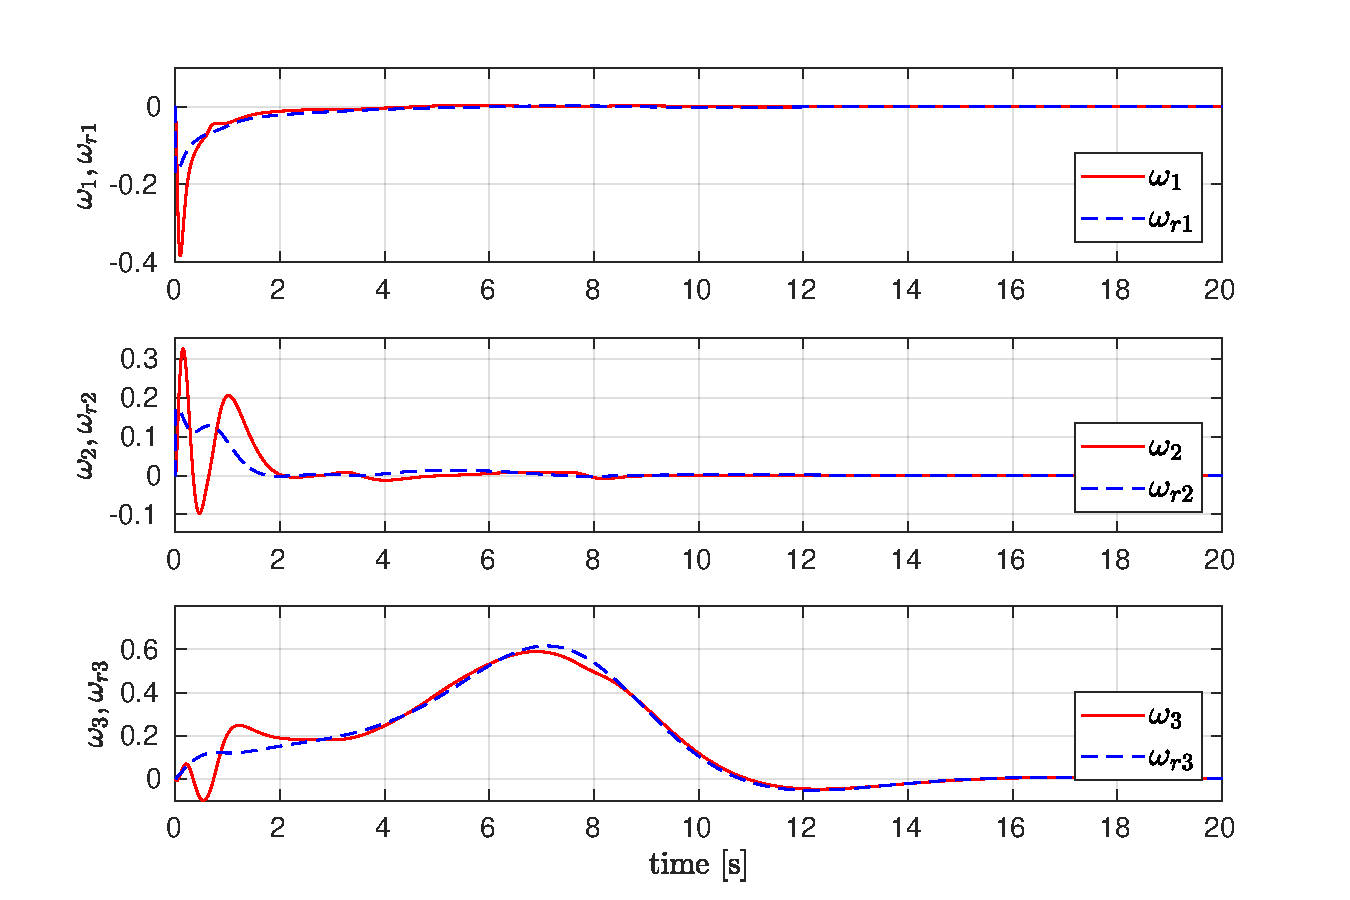
\includegraphics[width = 105mm]{Images/Data_avecCurrent_Om_Omr2.pdf}	
	\end{figure}
\end{block}
\end{frame}
\begin{frame}{Simulation results, \tiny$\mathbf{p}_C(0) = [-2, -1.5, -1 ]^{\top} (m)$, $\mathbf{R}(0) = \mathbf{R}_{\{\frac{\pi}{18},-\frac{\pi}{18},\pi\}}$, $\mathbf{V}(0) = \mathbf{\Omega}(0) = \mathbf{0}$}

\begin{block}{Current $\mathbf{V}_f = [\dfrac{1}{2\sqrt{2}}, \dfrac{1}{2\sqrt{2}}, 0] (m/s)$}
	\begin{figure}
		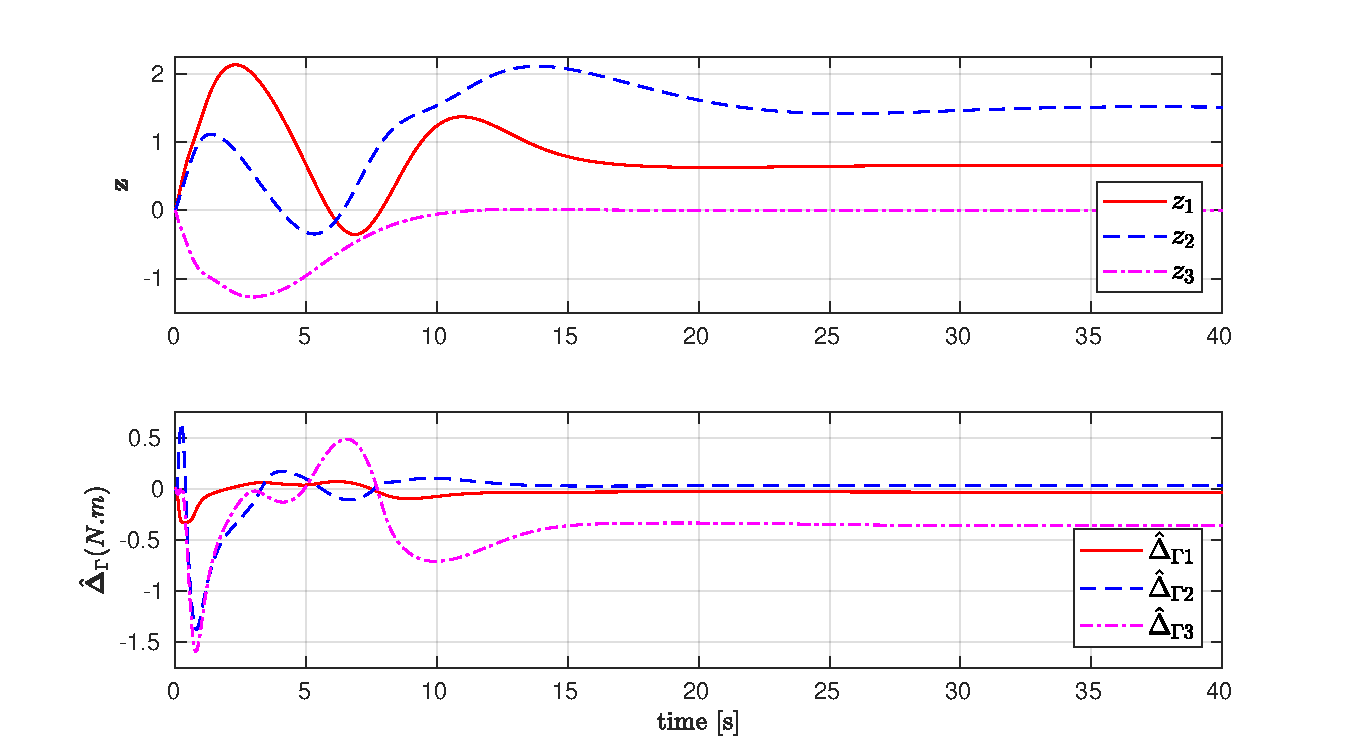
\includegraphics[width = 105mm]{Images/Data_avecCurrent_zep_hatDeltaG2.pdf}	
	\end{figure}
\end{block}
\end{frame}


% All of the following is optional and typically not needed. 
%\appendix
%\section<presentation>*{\appendixname}
%\subsection<presentation>*{For Further Reading}
%
%\begin{frame}[allowframebreaks]
%  \frametitle<presentation>{For Further Reading}
%    
%  \begin{thebibliography}{10}
%    
%  \beamertemplatebookbibitems
%  % Start with overview books.
%
%  \bibitem{Author1990}
%    A.~Author.
%    \newblock {\em Handbook of Everything}.
%    \newblock Some Press, 1990.
% 
%    
%  \beamertemplatearticlebibitems
%  % Followed by interesting articles. Keep the list short. 
%
%  \bibitem{Someone2000}
%    S.~Someone.
%    \newblock On this and that.
%    \newblock {\em Journal of This and That}, 2(1):50--100,
%    2000.
%  \end{thebibliography}
%\end{frame}

\end{document}


